\documentclass[11pt]{article}
\usepackage[utf8]{inputenc} % Para caracteres en espa�ol
\usepackage{amsmath,amsthm,amsfonts,amssymb,amscd}
\usepackage{multirow,booktabs}
\usepackage[table]{xcolor}
\usepackage{fullpage}
\usepackage{lastpage}
\usepackage{enumitem}
\usepackage{multicol}
\usepackage{fancyhdr}
\usepackage{mathrsfs}
\usepackage{wrapfig}
\usepackage[final]{pdfpages}
\usepackage{setspace}
\usepackage{esvect}
\usepackage{calc}
\usepackage{multicol}
\usepackage{cancel}
\usepackage{graphicx}
\graphicspath{ {pictures/} }
\usepackage[retainorgcmds]{IEEEtrantools}
\usepackage[margin=3cm]{geometry}
\usepackage{amsmath}
\newlength{\tabcont}
\setlength{\parindent}{0.0in}
\setlength{\parskip}{0.05in}
\usepackage{empheq}
\usepackage{framed}
%\usepackage{newtxmath}
\usepackage{euscript}
\DeclareMathAlphabet{\mathpzc}{T1}{pzc}{m}{it}
\usepackage[most]{tcolorbox}
\usepackage{xcolor}
\colorlet{shadecolor}{orange!15}
\parindent 0in
\parskip 12pt
\geometry{margin=1in, headsep=0.25in}
\theoremstyle{definition}
\newtheorem{defn}{Definition}
\newtheorem{reg}{Rule}
\newtheorem{exer}{Exercise}
\newtheorem{note}{Note}
\newcommand{\volume}{{\ooalign{\hfil$V$\hfil\cr\kern0.08em--\hfil\cr}}}
\newcommand{\parr}{\mathbin{\|}} % Parralel Symbol
\begin{document}
\setcounter{section}{0}
\setcounter{page}{5}
\setcounter{equation}{7}
\def\thepart{\arabic{part}}
\setcounter{part}{8}
\numberwithin{equation}{part}

 \pagestyle{fancy}
\fancyhf{}
\rhead{Section 8:  Electromagnetic Propulsion}
\rfoot{Page \thepage}
\thispagestyle{empty}

\begin{center}
{\LARGE \bf Section 8:  Electromagnetic Propulsion}\\
{\large AE435}\\
Spring 2018
\end{center}
\vspace{5mm}
\section{Coaxial Self-Field Thrusters}
\vspace{25mm}
\tableofcontents
\newpage
Schematic of a Magneto Plasma Dynamic (MPD) Accelerator: 

 \begin{center}
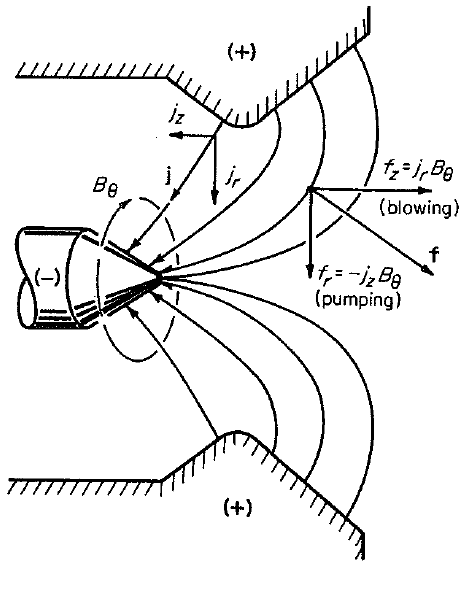
\includegraphics[scale=0.6]{4.png} 
\end{center}
Coaxial meaning the anode is surrounding the center-mounted cathode. We have a strong electric field between the anode and cathode which in turn forms an arc between the anode and cathode. The arc is passing through the plasma itself and that current creates a strong magnetic field. 

In other words, a "self-field" thruster is one where the magnetic field is due to the plasma current.  An "applied-field" thruster has a magnetic field that is externally applied (and will also have self-field too).
 
Can separate out two thrust components in a coaxial self-field thruster:
\begin{itemize}
\item \textbf{Blowing Forces}, which directly accelerate the gas in the axial direction
\item \textbf{Pumping Forces}, which provide a radial pressure gradient (and, thus, pressure thrust)
\end{itemize}
For axisymmetric current (no-theta component)
 \begin{equation}
 \begin{aligned}
 \nabla \times \vv{B} = \mu \, \vv{j}
 \end{aligned}
 \end{equation}
meaning the magnetic field is purely azimuthal.
  \begin{equation*}
 \begin{aligned}
 \vv{B} = B(r,z) \, \hat{\theta} \quad \text{Purely Azimuthal}
 \end{aligned}
 \end{equation*}
 \newpage
 \subsection{Blowing Contribution}
 \subsubsection{Cylindrical Cathode Tip}
To evaluate the blowing contribution, we can consider a simplified model:

 \begin{center}
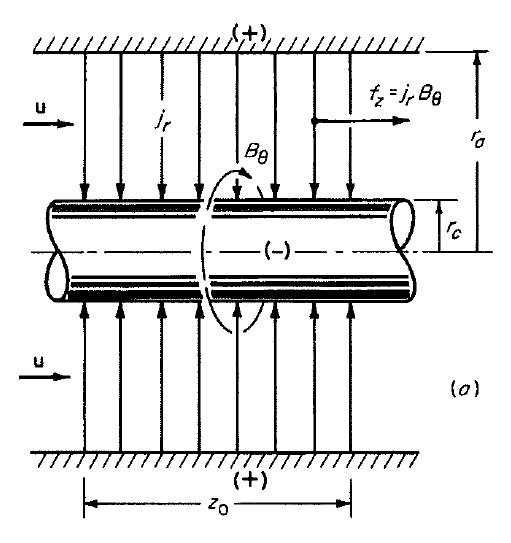
\includegraphics[scale=0.5]{5.png} 
\end{center}

If we assume a radial uniform current density $j_r$ at the cathode (as shown in the figure above), then
 
  \begin{equation}
 \begin{aligned}
 B_{\theta} (r,z) = \frac{\mu \, J}{2 \, \pi \, r} \, \bigg(1 - \frac{z}{z_o}\bigg)
 \end{aligned}
 \end{equation}
 
where $z_o$ is the length of the cathode and where the current into the cathode is:
 
  \begin{equation}
 \begin{aligned}
 J = \int_S \, \vv{j} \cdot \mathrm{d}\vv{A} = 2 \, \pi \, r \, z_o \, j_r
 \end{aligned}
 \end{equation}
 
which increases linearly with $z_o$.

The body force density in the axial direction is then:
 
  \begin{equation}
 \begin{aligned}
 f_z = j_r \, B_{\theta}
 \end{aligned}
 \end{equation}
 Combined with Equation 8.9
   \begin{equation}
 \begin{aligned}
 f_z = \frac{\mu \, J^2}{4 \, \pi^2 \, r^2 \, z_o^2} \, (z_o - z)
 \end{aligned}
 \end{equation}
 
To get the total force over the entire system we take the integral of the body force density over the gas volume:

  \begin{equation}
 \begin{aligned}
 F_z = \int_{0}^{z_o} \, \int_{0}^{2 \, \pi} \, \int_{r_c}^{r_a} \, f_z \, r \, \mathrm{d} r\, \mathrm{d}\theta \, \mathrm{d}z 
 \end{aligned}
 \end{equation}
 
Evaluating the thrust for this model:
 
  \begin{equation}
 \begin{aligned}
  F_z = \frac{\mu \, J^2}{4 \, \pi^2 \, z_o^2} \, \int_{0}^{z_o} \, \int_{0}^{2 \, \pi} \, \int_{r_c}^{r_a} \, \frac{(z_o - z)}{r^2} \mathrm{d} r\, \mathrm{d}\theta \, \mathrm{d}z 
 \end{aligned}
 \end{equation}
 
yields
 \begin{shaded}
 \textbf{Cylindrical-Tipped Cathode Thrust:}
 
  \begin{equation}
 \begin{aligned}
 F_z = \frac{\mu \, J^2}{4 \, \pi} \, \ln \bigg(\frac{r_a}{r_c}\bigg) 
 \end{aligned}
 \end{equation}
 \end{shaded}

This is the total blowing (axial) force when we have a cylindrical cathode. There is no pinching or pumping force for a cylindrical cathode. Notice it is dependent on $J^2$ which would make sense. If we were to increase the current, we would expect to get a larger force. It is also dependent on the geometry, the cathode and anode radius.
 
 \subsubsection{Conical Cathode Tip}
You can model a conical tip cathode the same way:

 \begin{center}
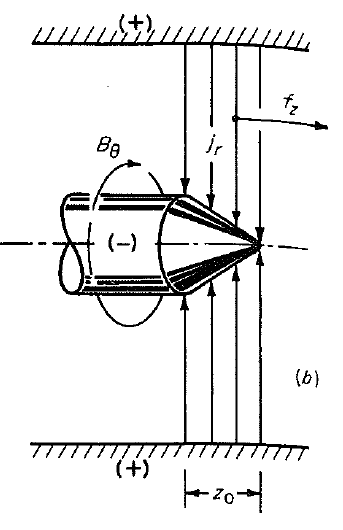
\includegraphics[scale=0.5]{6.png} 
\end{center}

If we assume a uniform current density $j_a$ at the anode, then the cathode current density varies inversely with cathode radius (as the current increases, the radius must decrease).  The new volume integral
 
  \begin{equation*}
 \begin{aligned}
  F_z = \int_{0}^{z_o} \, \int_{0}^{2 \, \pi} \, \int_{r_c \, (1-\frac{z}{z_o})}^{r_a} \, f_z \, r \, \mathrm{d} r\, \mathrm{d}\theta \, \mathrm{d}z 
 \end{aligned}
 \end{equation*}
 
yielding...

  \begin{shaded}
 \textbf{Conical-Tipped Cathode Thrust for Uniform Anode Current Density:}
  \begin{equation}
 \begin{aligned}
  F_z = \frac{\mu \, J^2}{4 \, \pi} \, \ln \bigg(\frac{r_a}{r_c} + \frac{1}{2}\bigg) 
 \end{aligned}
 \end{equation}
 \end{shaded}
If we assume a uniform current density $j_c$ at the cathode, then we get:
 
  \begin{shaded}
 \textbf{Conical-Tipped Cathode Thrust for Uniform Cathode Current Density:}
  \begin{equation}
 \begin{aligned}
  F_z = \frac{\mu \, J^2}{4 \, \pi} \, \ln \bigg(\frac{r_a}{r_c} + \frac{1}{4}\bigg) 
 \end{aligned}
 \end{equation}
 \end{shaded}
Either way, current flow to a conical cathode tip increases the blowing force compared with a cylindrical cathode (Equation. 8.15).  In coaxial thrusters with long solid-rod cathodes, the tip current fraction is $\sim10\%$.
 \newpage
 \subsection{Pumping Contribution}
To evaluate the pumping contribution, consider another simple model:

 \begin{center}
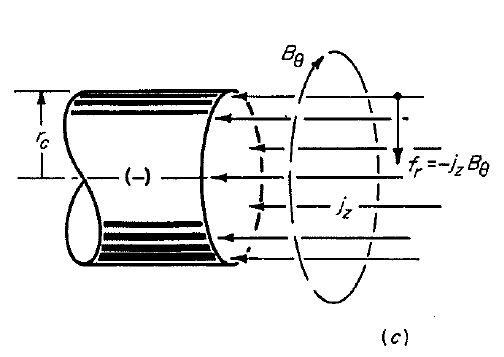
\includegraphics[scale=0.6]{7.png} 
\end{center}

Here, all the current enters the face of the cathode, and the magnetic field becomes (as we saw within the arc column, Equation 7.76):
 
  \begin{equation}
 \begin{aligned}
 B_{\theta} (r,z) = \frac{\mu \, J^2 \, r}{2 \, \pi \, r_c^2}
 \end{aligned}
 \end{equation}
The radial force density 

  \begin{equation}
 \begin{aligned}
 f_r = j_z \, B_{\theta} = \frac{\mu \, J^2 \, r}{2 \, \pi^2 \, r_c^4} = - \frac{\partial p}{\partial r}
 \end{aligned}
 \end{equation}
 
is balanced by the radial pressure gradient, $\frac{\partial p}{\partial r}$.

Integrating over r, you get a parabolic pressure profile:
 
  \begin{equation}
 \begin{aligned}
 p(r) = p_o + \frac{\mu \, J^2}{4 \, \pi^2 \, r_c^2} \, \Bigg[1 - \bigg(\frac{r}{r_c}\bigg)^2\Bigg]
 \end{aligned}
 \end{equation}
 
which can be integrated over the cathode tip to give a pressure force.
 
  \begin{equation}
 \begin{aligned}
 F_c = 2 \, \pi \, \int_0^{r_c} \, (p - p_o) \, r \, \mathrm{d}r = \frac{\mu \, J^2}{8 \, \pi}
 \end{aligned}
 \end{equation}
 
 $p$ is the pressure in the arc while $p_o$ is the ambient pressure. To get the total force, we add up the blowing and pumping contributions. 
 
  \subsection{Maecker Model}
A more general model, including all of the above:

 \begin{center}
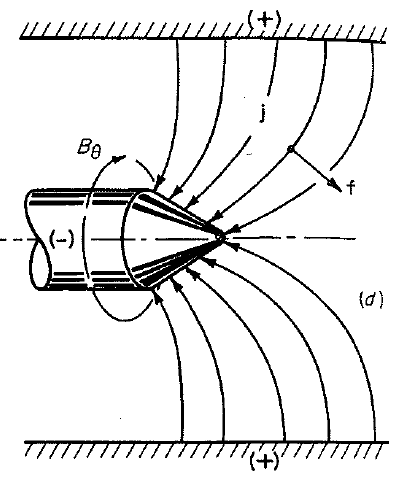
\includegraphics[scale=0.6]{8.png} 
\end{center}

Adding together all the blowing and pumping contributions, gives:
 \begin{shaded}
 \textbf{Maecker Formula}
  \begin{equation}
 \begin{aligned}
  F = \frac{\mu \, J^2}{4 \, \pi} \, \Bigg(\ln \bigg(\frac{r_a}{r_c}\bigg) + \frac{3}{4}\Bigg)
 \end{aligned}
 \end{equation}
 \end{shaded}
 
This is the Maecker formula, derived in 1955.
\begin{itemize}
\item Thrust is independent of flow rate and current flow details. The only thing that matters is the current, $J$, and the geometry.
\item The specific impulse varies as, $\frac{J^2}{\dot{m}}$ 
\end{itemize}
\begin{framed}
Proof:
  \begin{equation*}
 \begin{aligned}
 I_{SP} = \frac{F}{g_o \, \dot{m}} = \frac{\mu \, J^2}{4 \, \pi \, g_o \, \dot{m}} \, \Bigg(\ln \bigg(\frac{r_a}{r_c}\bigg) + \frac{3}{4}\Bigg)
 \end{aligned}
 \end{equation*}
 \end{framed}
 \newpage
\textbf{How well does Maecker compare to real thruster data?}

First we define a thrust coefficient:
 
  \begin{equation}
 \begin{aligned}
 C_T = \frac{4 \, \pi}{\mu_o} \, \frac{F}{J^2}
 \end{aligned}
 \end{equation}
 
so that thrust
 
  \begin{equation*}
 \begin{aligned}
 F = C_T \, \frac{\mu_o}{4 \, \pi} \, J^2
 \end{aligned}
 \end{equation*}
 
Notice that for the Maecker formula, $C_T$ is a constant for a particular geometry:
 
What this model is essentially saying then is that once I have built my thruster (such that all geometries are fixed), when I run my thruster and change the current input, there is no change in the thrust coefficient. My thrust coefficient does not change. In the figure below, the Maecker formula is constant and stays constant. We see that it models the thrust coefficient almost close for high current states but fails when operating at lower currents. 
  
 \begin{center}
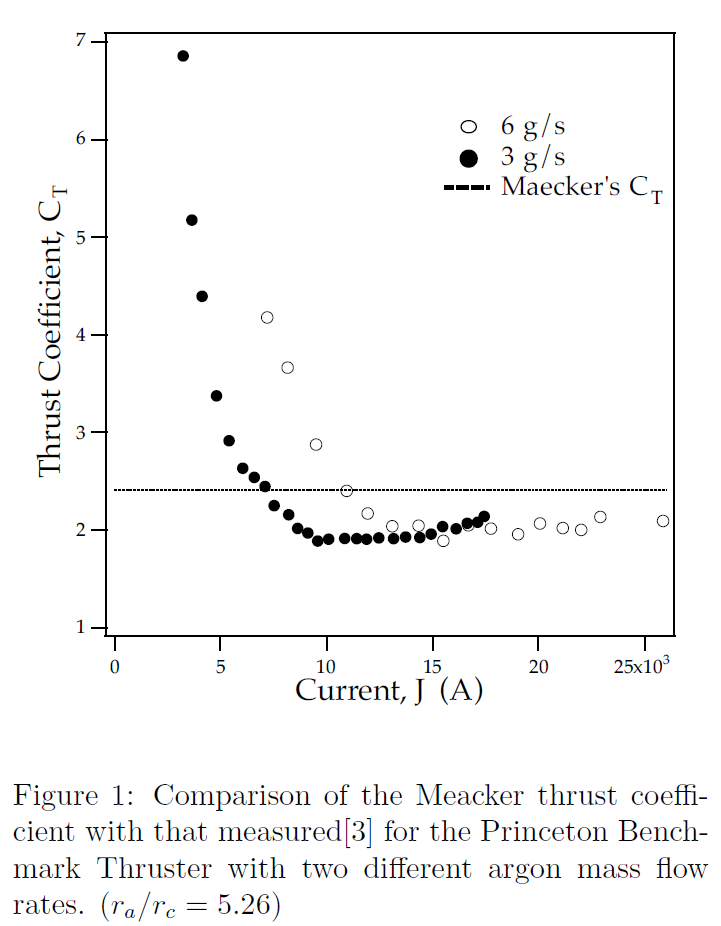
\includegraphics[scale=0.5]{9.png} 
\end{center}

 
The actual data (from Choueiri, "On the Thrust of Self-field MPD Thrusters", IEPC-97-121, 1997) comparison with the Princeton Benchmark Thruster (PBT):
\begin{itemize}
\item Is generally much lower than the Maecker $C_T$ at high J
\item Much higher than the Maecker $C_T$ at low J
\item Shifts with mass flow rate
\end{itemize}
Why are we seeing this?
\begin{itemize}
\item \textbf{Traditional Explanation:}  Electrothermal component of thrust.  We are heating up the gas! In other words, we don't have just electromagnetic force ($J\times B$),  we also have some electrothermal acceleration. If we look at the geometry, the anode has a converging diverging shape so we will have some type of electrothermal component to it. But it is hard to see why thrust would decrease with increasing J? A better explanation...
\item \textbf{Modern:}  Pumping forces on the rear of the chamber.  Not much experimental verification yet, but Choueiri's model (which includes all surfaces) does pretty well.
\end{itemize}
\newpage
  \subsection{Tikhonov Model}
Tikhonov (1976) came up with an improvement on the Maecker model.
Assumptions:
\begin{itemize}
\item Quasi 1-D flow
\item Single-fluid single-temperature MHD plasma
\item Isothermal fluid
\item High Magnetic Reynolds Number (plasma carries magnetic field with it as it convects)
\end{itemize}

Model:
  \begin{equation}
 \begin{aligned}
 C_T = \frac{\gamma+1}{2} + \frac{\alpha_o^{-2}}{2}
 \end{aligned}
 \end{equation}
 
The dimensionless parameter $\alpha_o$	is given by:
 
  \begin{equation*}
 \begin{aligned}
 \alpha_o = \frac{\gamma \, \mu_o}{8 \, \pi \, a_o} \, \frac{J^2}{\dot{m}}
 \end{aligned}
 \end{equation*}
 
where
 \begin{equation*}
 \begin{aligned}
 \gamma &= \text{Adiabatic Index} \\ \\
 a_o = \sqrt{\gamma \, R \, T} &= \text{Speed of Sound}
 \end{aligned}
 \end{equation*}
 
 Notice how that the results are independent of geometry, $\frac{r_a}{r_c}$. There is also no model for ionization potential $\varepsilon_i$. So if we were to switch gases, there is no accounting for how the ionization potential changes for the type of gas being used. 
\newpage
However, it does a better job than the Maecker Formula of following the general trend of the data:

 \begin{center}
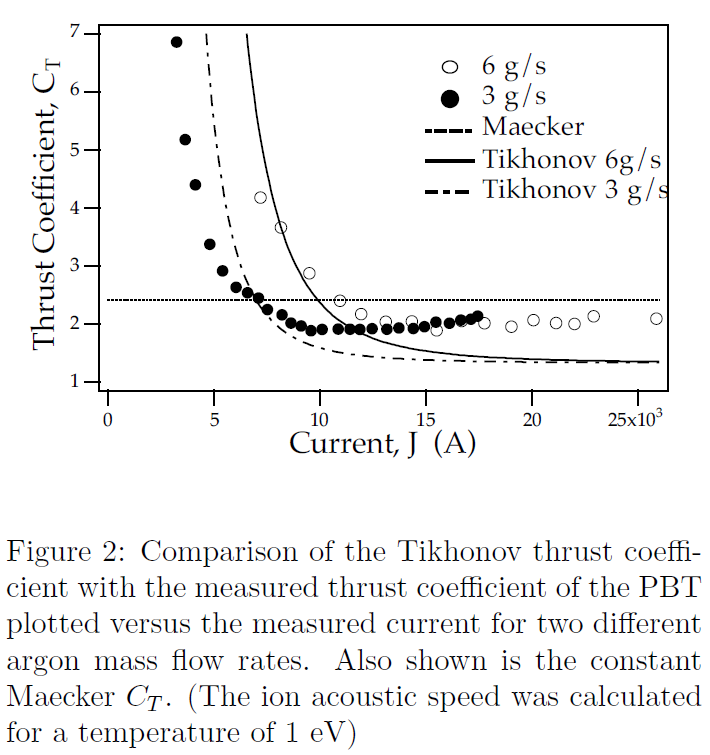
\includegraphics[scale=0.6]{10.png} 
\end{center}

Unfortunately, when   $\frac{J^2}{\dot{m}}$   	is high, the Tikhonov formula predicts that:
 
  \begin{equation}
 \begin{aligned}
 C_T \cong \frac{\gamma+1}{2}
 \end{aligned}
 \end{equation}
 
meaning that for       $\gamma \gg 1$         	this model seriously under-predicts the high-thrust,        $\frac{J^2}{\dot{m}}$.
 \newpage
  \subsection{Choueiri Model}
Choueiri (1997) came up with the best model yet where we are basically calculating the force on all of the surfaces of the control volume.

First-principles model of the Princeton Benchmark Thruster:

 \begin{center}
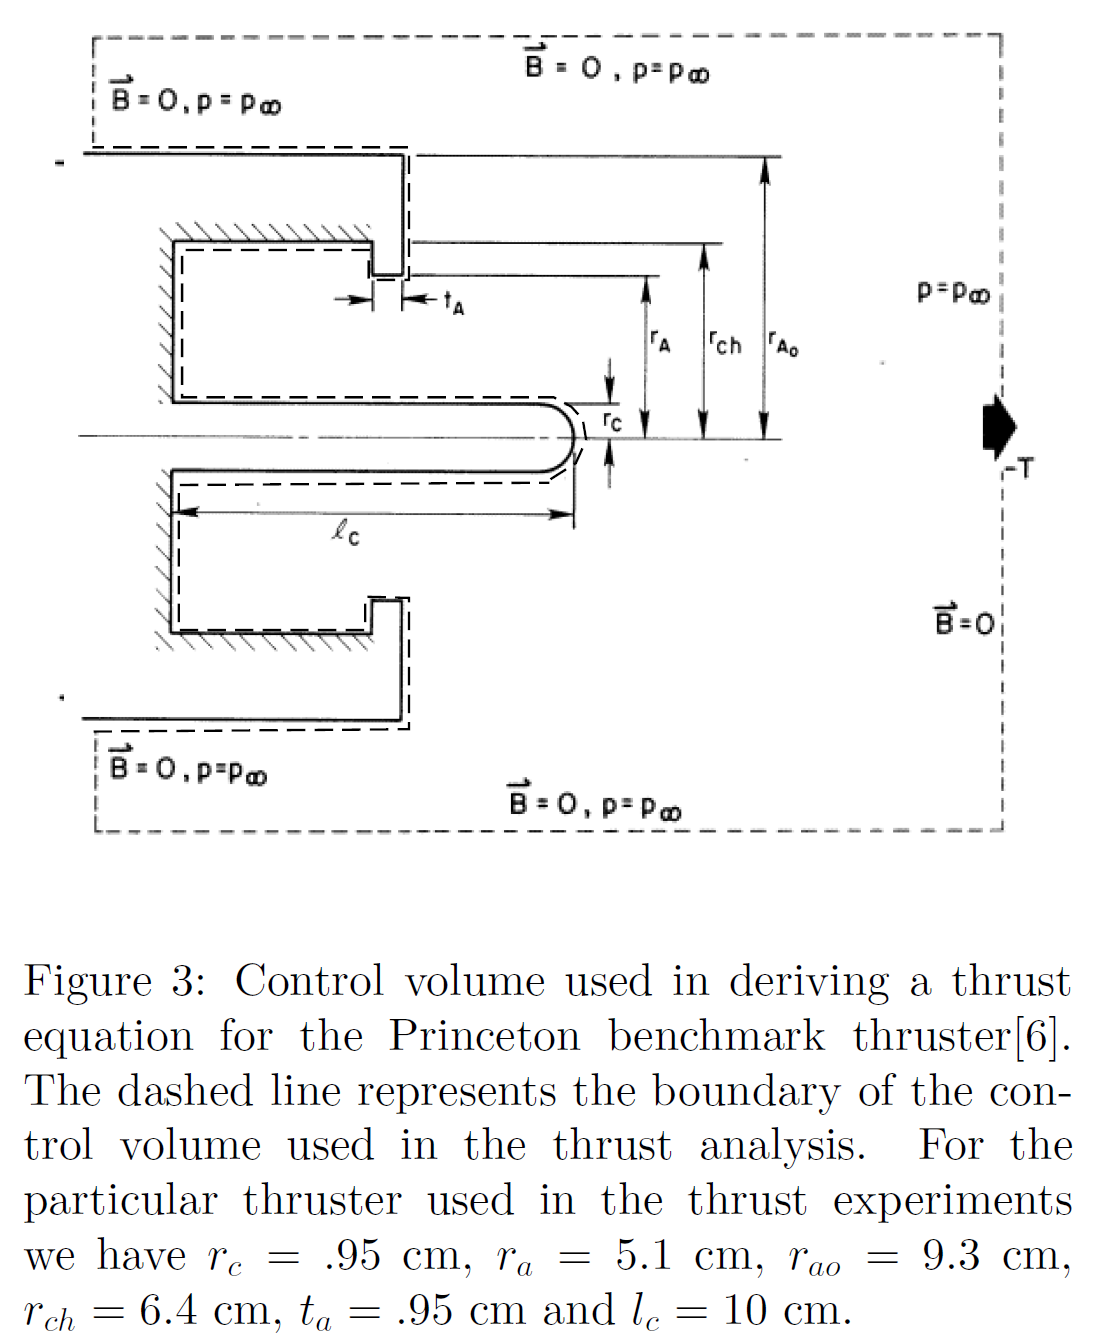
\includegraphics[scale=0.4]{11.png} 
\end{center}

Choueiri considers the Blowing (b) and Pumping/Pinching (p) contributions from the:
\begin{itemize}
\item Backplate (BP)
\item Anode inner face (AIF)
\item Anode outer face (AOF)
\item Cathode tip (CT)
\end{itemize}

Each of these curves in the Figure 6 below represents the individual contributions from each of the surfaces listed above. If we add all of the pinching and blowing contributions on all of the surfaces, we arrive at a sum or total thrust coefficient, $C_T$, that closely matched experimental data. 

 \begin{center}
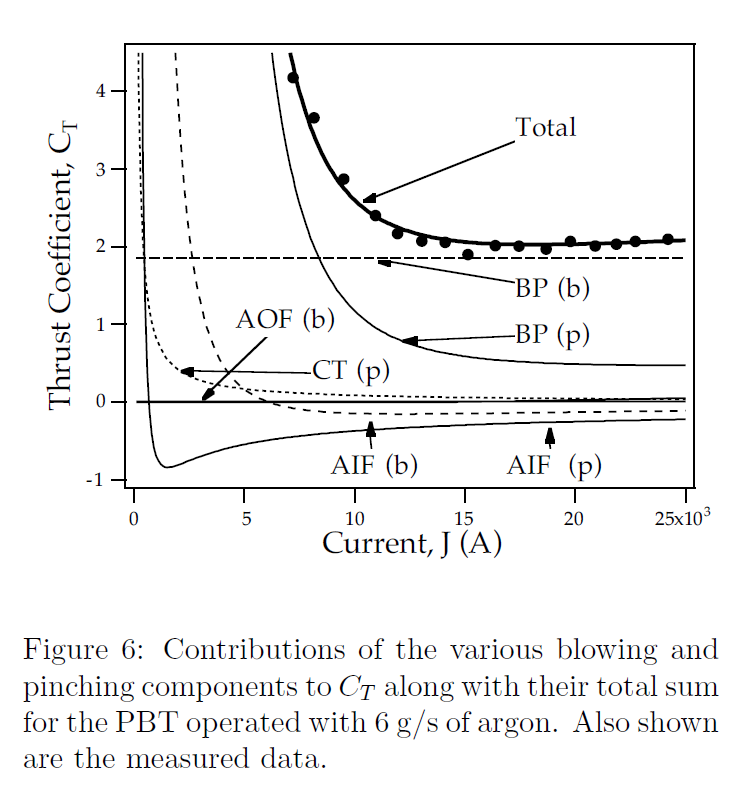
\includegraphics[scale=0.6]{12.png} 
\end{center}

To scale this to other thrusters, Choueiri looked at how ionization sucks energy away from useful work (plasma acceleration).  When the jet power equals the ionization energy loss rate:
  \begin{equation}
 \begin{aligned}
 \frac{1}{2} \, F \, u_e = \dot{m} \, \frac{\varepsilon_i}{M}
 \end{aligned}
 \end{equation}
where
 \begin{equation*}
 \begin{aligned}
\varepsilon_i &= \text{Ionization Energy} \\
M &= \text{Heavy-Particle (Ion or Neutral) Mass}
 \end{aligned}
 \end{equation*}

We can solve for a critical ionization speed
 \begin{shaded}
 \textbf{Critical Ionization Speed}
  \begin{equation}
 \begin{aligned}
 u_{ci} = \bigg(\frac{2 \, \varepsilon_i}{M}\bigg)^{\frac{1}{2}}
 \end{aligned}
 \end{equation}
 \end{shaded}
Where we can use values for typical propellants experimentally collected or known:
 \begin{center}
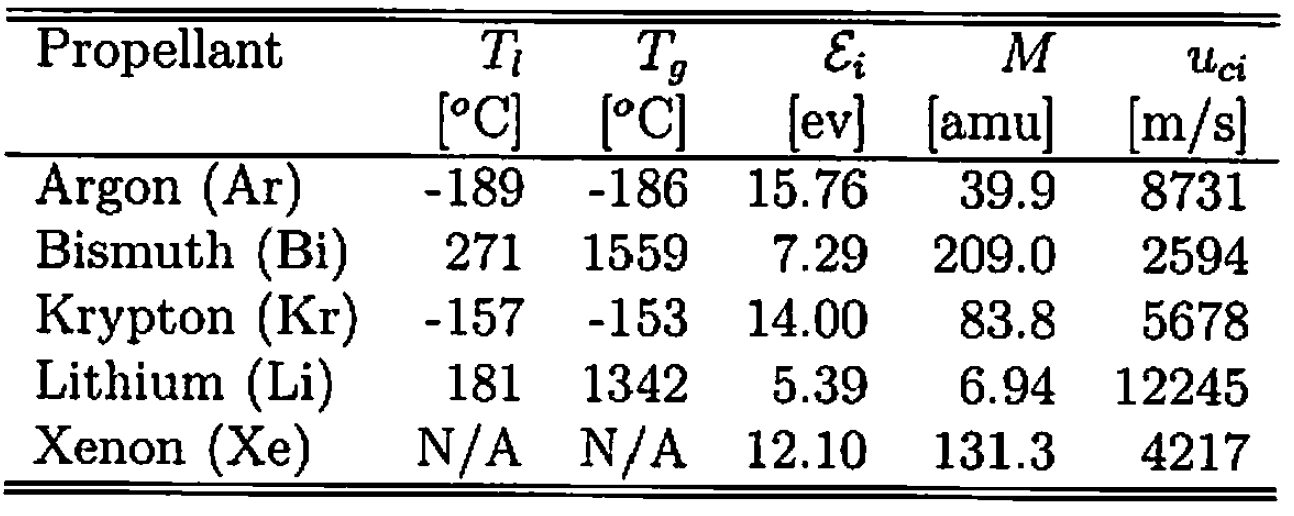
\includegraphics[scale=0.4]{13.png} 
\end{center}
We can nondimensionalize J as:
  \begin{equation}
 \begin{aligned}
 \xi = \frac{J}{J_{ci}}
 \end{aligned}
 \end{equation}
Where a critical current is defined as, 
  \begin{equation}
 \begin{aligned}
 J_{ci} = \bigg(4 \, \pi \, \frac{\dot{m} \, u_{ci}}{\mu_o \, C_T}\bigg)^{\frac{1}{2}}
 \end{aligned}
 \end{equation}

which relates                        $u_{ci}$        to $C_T$ and $J$.                   Using the Maecker approach, the dimensionless current can be expressed as:
 \begin{shaded}
 \textbf{Dimensionless Current}
  \begin{equation}
 \begin{aligned}
 \xi = \frac{J \bigg(\frac{\mu_o}{4 \, \pi}\,\ln\big(\frac{r_a}{r_c}\big)\bigg)^{\frac{1}{2}}}{\dot{m}^{\frac{1}{2}}\bigg(\frac{2 \, \varepsilon_i}{M}\bigg)^{\frac{1}{4}}}
 \end{aligned}
 \end{equation}
 \end{shaded}
This formulation has been shown to relate thruster performance pretty well to propellant mass and ionization energy. As such, Choueiri derived the following scaling laws for $C_T$:

\begin{framed}
\textbf{Choueiri Scaling Laws for \bf{$C_T$}}
  \begin{equation*}
 \begin{aligned}
 C_T &\sim \xi^{-4} \qquad &\qquad \text{for } \xi < 1 \\
   C_T &\sim \ln\bigg(\frac{r_a}{r_c} + \xi^2 \bigg) \qquad & \qquad \text{for } \xi > 1 \\
 \end{aligned}
 \end{equation*}
 \end{framed}
 
which can be combined into a single formula as:
 \begin{shaded}
 \textbf{Choueiri Scaling Law for \bf{$C_T$}}
  \begin{equation}
 \begin{aligned}
 C_t = \frac{\nu}{\xi^4} + \ln\bigg(\frac{r_a}{r_c}+ \xi^2 \bigg)
 \end{aligned}
 \end{equation}
where
 \begin{equation*}
 \begin{aligned}
 \nu = \frac{\dot{m}}{\dot{m^*}}
 \end{aligned}
 \end{equation*}
 \end{shaded}
 From 6 g/s argon data, the scaling flow rate is derived to be:
 \begin{shaded}
 \textbf{Scaling Flow Rate}
  \begin{equation*}
 \begin{aligned}
 \dot{m^*} = 66 \quad [g/s]
 \end{aligned}
 \end{equation*}
 \end{shaded}
This scaling flow rate is not a theoretical model. It is a scaling model based on data from Argon but we take it to be $66 \, [g/s]$ for all gases that we work with. 
 \newpage
Figure 7 in Choueiri shows how this scaling method (not quite a model) applies to argon and xenon data.
 
 \begin{center}
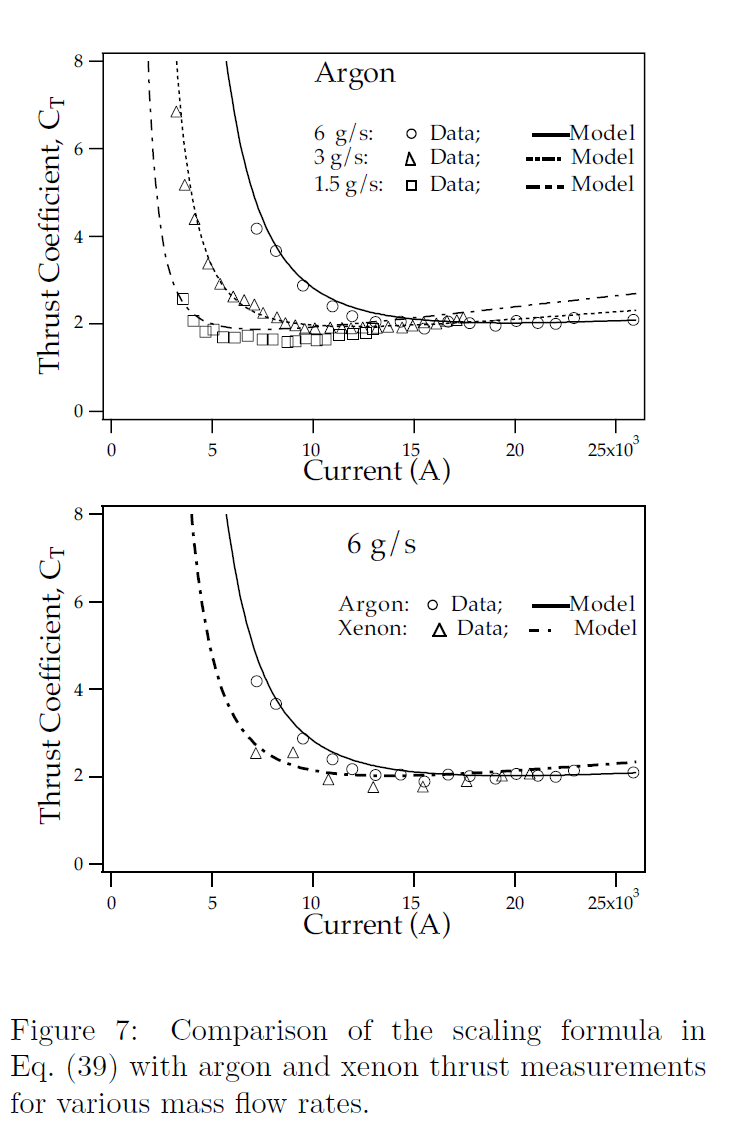
\includegraphics[scale=0.7]{14.png} 
\end{center}

\subsection{Power Analysis}
  \begin{equation}
 \begin{aligned}
P_e = \frac{1}{2} \, F \, u_e = J^2 \, Z
 \end{aligned}
 \end{equation}
 
 Use impedance Z instead of ohmic resistance R because propulsion systems can have reactive elements (capacitance, inductance) in addition to resistance.
 
 Thus, for T=F of Maecker Formula (Equation 8.22)...
   \begin{equation}
 \begin{aligned}
Z = \frac{F \, u_e}{2 \, J^2} = \frac{1}{2} \, \frac{\mu_o }{4 \, \pi} \, \bigg[ \ln \Big(\frac{r_a}{r_c} \Big) + \frac{3}{4}\bigg] \, u_e = \frac{1}{2} \, k \, u_e
 \end{aligned}
 \end{equation}

\begin{framed}
\textbf{Example: } Consider a system with an exit velocity of 40,000 m/s, an anode to cathode ratio of 5 and a current of 20 kA. Find the Thrust, Exit Jet Power, Impedance and Voltage for this system.

We have:
   \begin{equation*}
 \begin{aligned}
u_e &= 40000 \quad [m/s] \qquad , \qquad
\frac{r_a}{r_c} &\sim 5 \qquad , \qquad 
J &= 20 \quad [kA]
 \end{aligned}
 \end{equation*}
 
 We can find the thrust using Equation 8.22.
 
    \begin{equation*}
 \begin{aligned}
F = \frac{\mu \, J^2}{4 \, \pi} \, \Bigg(\ln \bigg(\frac{r_a}{r_c}\bigg) + \frac{3}{4}\Bigg) = 94.4 \, [N]
 \end{aligned}
 \end{equation*}
 
 Leading us to now find...
     \begin{equation*}
 \begin{aligned}
P_e &= \frac{1}{2} \, F \, u_e = 1.9\times10^6 \, [W] \\ \\
Z &= 0.00472 \, [\omega] \\ \\
V &= J \, Z = 94.4 \, [Volts] 
 \end{aligned}
 \end{equation*}
 
 This is a fairly low voltage! The actual voltage of the system will be higher since ohmic resistance (due to $\omega_o$) and voltage sheaths not included.
 \end{framed}


\end{document}